\subsubsection{Tile Parameter Exploration}
We use three levels of tiling in our optimization. The size of the first-level tile depends on the second input sequence, which is a program parameter. That leaves us to explore second and third-level tiling parameters. We choose matrix-max plus operation on two matrices of size $M \times K$ and $K \times N$ to explore the best register tile and mono-parametric tile parameter. We choose square matrices $(M = N = K = 2800)$ such that the footprint exceeds the L3 cache.
Figure~\ref{fig:register_tile_performance_comparison} compares performance between different register tiles on Coffee Lake. We tile the three outer loops $M$, $K$, and $N$ with a mono-parametric tile size of $192$. Then, we register-tile each patch. The register-tile kernel assumes that the data is accessed sequentially. All the results shown here include the packing operation of these patches.
\begin{figure}[htbp]
    \centering
    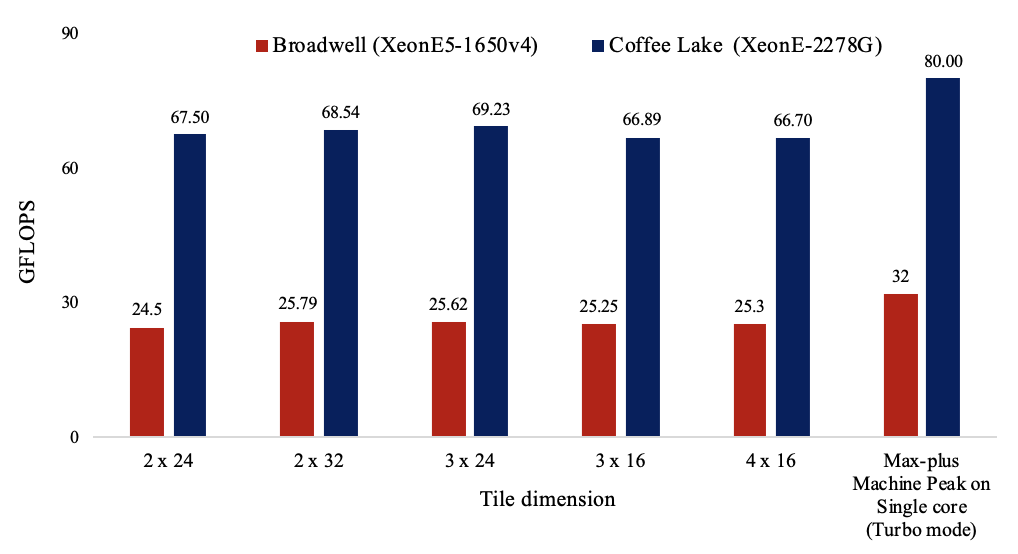
\includegraphics[scale=0.4, trim=4 4 4 4,clip]{content/figures/max_plus_register_tile_performance.png}
   \caption{Register Tiled Matrix max-plus Performance Comparisons. $M = K = N = 2880$, $N_{tile}= 192$}
\label{fig:register_tile_performance_comparison}
\end{figure}
We notice that the register-tile $3 \times 24$ performs the best which matches our theoretical register allocation strategy. 
To explore second-level tile size, we fixed the register tile parameters and vary the second-level tile size [48, 72, 120, 192]. We find that the second-level tile size of 48 performs better than the others for double max-plus and BPMax when the register-tile size is $3 \times 24$. When $N_{tile}=48$, all the inputs and outputs of the register-tiled kernel fit in the $L_{1}$. So, we use $N_{tile}=48$ and register-tile dimension of $3 \times 24$ for the rest of our experiments.
